

\chapter{Operating Systems}
\label{chap:operating-systems}

In this chapter we provide a survey of existing operating systems and mechanisms for building
mixed-criticality systems. Although not all operating systems support mixed-criticality, we evaluate
the scheduling and resource sharing policies and mechanisms available, with a focus on temporal isolation,
asymmetric protection, and resource sharing. 

% TODO update
First, we look at the \gls{POSIX} standard which impacts many commercial and open source operating
systems. Then we examine what is available in Linux and survey existing relevant operating systems
from the open source community, research and commercial \glspl{OS}. We then examine deeper isolation
and resource sharing techniques and how they interact with capability systems.

\section{POSIX}

The \gls{POSIX} standard specifies \gls{RTOS} interfaces~\citep{Harbour_93} which
influence a large amount of \gls{OS} design.  Scheduling policies specified by \gls{POSIX} are shown in
\Cref{tab:posix-sched}. 

\begin{table}
\centering
\rowcolors{2}{gray!25}{white}
\begin{tabular}{lp{.7\textwidth}}\toprule
    \emph{Policy}  & \emph{Description} \\\midrule
    \schedfifo     & Real-time tasks can run at a minimum of 32 fixed-priorities until they are preempted or yield. \\
    \schedrr       & As per \schedfifo but with an added timeslice. If the timeslice for a thread expires, it is added to the tail of the scheduling queue for its priority.\\
    \schedsporadic & Specifies sporadic servers as described in \Cref{p:sporadic} and can be used
    for temporal isolation. For practical requirements, the POSIX specification of \schedsporadic
    specifies a maximum number of replenishments which is implementation defined. \\\bottomrule
\end{tabular}
\caption{\gls{POSIX} real-time scheduling policies}
\label{tab:posix-sched}
\end{table}

\citet{Faggioli_08} provides an implementation of \schedsporadic, which \citet{Stanovic_BWH_10}
use to show that the POSIX definition of the sporadic server is incorrect and can allow tasks to
exceed their utilisation bound.  The authors provide a modified algorithm for merging and abandoning
replenishments which fixes these problems, of which corrections to the pseudo code were published in
\citet{Danish_LW_11}.  In further work \citet{Stanovic_BW_11} show that while sporadic servers
provide better response times than polling servers under average load, under high load the overhead
of preemptions due to fine-grained replenishments causes worse response times when compared to
polling servers.  Consequently they evaluate an approach where servers alternate between sporadic
and polling servers depending on load, where the transition involves reducing the maximum number of
replenishments to one and merging available refills.

Resource sharing in the \gls{POSIX} \gls{OS} interface is permitted through mutexes, which can be
used to build higher synchronisation protocols.  \Cref{tab:posix-mutex} shows the specified
protocols. 

\begin{table}
\centering
\rowcolors{2}{gray!25}{white}
\begin{tabular}{lp{.7\textwidth}}\toprule
\emph{Policy} & \emph{Description} \\\midrule
\noprioinherit & Standard mutexes that do not protect against priority inversion. \\
\prioinherit  & Mutexes with \gls{PIP} to prevent priority inversion, recall \Cref{sec:pip}. \\
\prioprotect & Mutexes with \gls{HLP} to prevent priority inversion, recall \Cref{sec:hlp}. \\
\bottomrule
\end{tabular}
\caption{\gls{POSIX} real-time mutex policies for resource sharing.}
\label{tab:posix-mutex}
\end{table}

Although \gls{POSIX} provides \schedsporadic which can be used for temporal isolation (however
flawed), the intention of the policy is to contain aperiodic tasks.  Since \schedsporadic allows
tasks to run at a lower priority when they have exceeded their allowed budget in any given period,
it follows that the locking protocols \prioinherit and \prioprotect would continue to operate --
although the excess time is not billed to the task.  If a task never releases a locked resource,
temporal isolation is completed violated.  As a result, \gls{POSIX} is insufficient for
mixed-criticality systems where tasks of different criticalities share resources.  Few \glspl{OS}
implement the full \gls{POSIX} standard, however many incorporate features of it, including Linux.

\section{Existing operating systems}

Here we provide a survey of existing open source, research and commercial operating systems with
real-time mechanisms. 

\subsection{Open source}

\paragraph{Linux} While Linux cannot be considered a real-time operating system for high criticality applications, it
is frequently used for lower criticality applications with \gls{SRT} demands.  Additionally, Linux
is often used as a platform for conducting real-time systems research. 
% TODO cite completely fair scheduler
Linux has fixed-priority preemptive scheduler which is split into scheduling classes.  Real-time
threads can be scheduled with \gls{POSIX} \schedfifo and \schedsporadic. Best effort threads are
scheduled with \gls{CFS}, and real-time threads are scheduled either \gls{FIFO} or round-robin, and
are prioritised over the best effort tasks.  Fixed priority threads in Linux are completely trusted:
apart from a bound on total execution time for real-time threads which guarantees that best effort
threads are scheduled (referred to as real-time throttling~\citep{Corbet_08}), individual temporal
isolation is not possible.

Linux version 3.14 saw the introduction of an \gls{EDF} scheduling class to Linux~\citep{Corbet_09},
which is between the fair and the fixed priority scheduling classes.  The \gls{EDF} implementation
allows threads to be temporally isolated using \gls{CBS}.

Scheduling in Linux promotes the false correlation we see in many systems: real-time tasks are
automatically trusted (unless scheduled with \gls{EDF}) and assumed to be more important, or more
critical, than best effort tasks.  In reality, criticality and real-time strictness are orthogonal.
Linux does not provide any mechanisms for asymmetric protection beyond priority.

On the resource sharing side Linux provides real-time locking via the POSIX  as per
\Cref{tab:posix-mutex}.

A large amount of projects exist that attempt to retrofit more extensive real-time features onto
Linux.  We briefly summarise major and relevant works here.  One of the original
works~\citep{Yodaiken_Barabanov_97} runs Linux as a fully preemptable task via virtualisation and
kernel modifications.  Interrupts are handled by the virtualisation layer, and only directed to
Linux if required.  This means that real-time tasks do not have to suffer from long interrupt
latencies, however it also means that devices drivers need to be rewritten from scratch for
real-time.

\litmus~\citep{Calandrino_LBDA_07} is an extension of Linux that allows for pluggable real-time
schedulers to be easily developed for testing multiprocessor schedulers.

Linux/RK~\citep{Oikawa_Rajkumar_98} is a resource kernel implementation Linux that is often used to
implement new scheduling algorithms.  \gls{ZS} scheduling~\citep{deNiz_LR_09} was implemented and
tested using Linux/RK.

Whilst Linux implementations are suitable for implementing algorithms, being used as test-beds and
even being deployed for non-critical \gls{SRT} applications, ultimately Linux is not a suitable
\gls{RTOS} for running safety-critical \gls{HRT} applications. The large amount of source code
results in a colossal trusted computing base,where it is impossible to guarantee correctness through
formal verification or timeliness through {\gls{WCET}} analysis.  Major reasons for adapting Linux
to real-time are the existing applications and wide array of device and platform support. For
mixed-criticality systems these advantages can be leveraged by virtualising Linux to run \gls{SRT}
and best effort applications.

\paragraph{RTEMS}~\citep{RTEMS:URL} is an open-source \gls{RTOS} that operates with or without
memory protection, although in either case it is statically configured.  Although it is an open
source project, RTEMS is used widely in industry and research.  The main scheduling policy is
\gls{FPRM}, however \gls{EDF} is also available with temporal isolation an option using \gls{CBS}.
No temporal isolation mechanisms are present for fixed-priority scheduling.  RTEMS provides
semaphores with \gls{PIP} or \gls{HLP} for resource sharing, as well as
higher level primitives for these. 

\paragraph{FreeRTOS}~\citep{FreeRTOS:URL} is another open-source \gls{RTOS}, however it only supports systems with \glspl{MPU}, not
\glspl{MMU}. The scheduler is preemptive \gls{FP} and \gls{PIP} is provided to avoid priority inversion.
FreeRTOS can be configured to be tickless or not.

\subsection{Research OSes}

\paragraph{Real-time Mach}~\citep{Mercer_RZ_94, Mercer_ST_93} first introduced the concept of
processor capacity reserves which implemented \gls{DS}. Mach used a fixed-priority, two level 
scheduler where threads with reserves would execute first, then threads without reserves and with
depleted reserves would be scheduled using a second level time-sharing scheduler.
An admission test was conducted in the kernel when reservations were created. 
Finally, Real-time Mach provided \gls{PIP} to avoid priority inversion~\citep{Tokuda_NR_90}.

\paragraph{EROS}~\citep{Shapiro_SF_99} is a capability based operating system designed to
demonstrate the viability of capability-based systems in terms of performance.  EROS introduced the
idea of a single-use reply capability, termed a \emph{resume} capability, which when invoked would
be consumed and allows the receiver to reply to the sender.  EROS also used what is known as an
\emph{entry} capability, which allowed the holder to invoke the services provided by a program
within a particular process.  EROS uses the same scheduling and resource sharing policies as
Real-time Mach, using capacity reserves, however these are not accessed via the capability system.

\paragraph{DROPS} (Dresden Real-time OPerating System)~\citep{Haertig_BBHHMRSW_98} is an L4 based
real-time microkernel that also takes the resource reservation route to temporal isolation.  The
scheduling scheme in DROPS allows a process to reserve a priority for an amount of cycles during a
time period.  Page colouring is used to reserve parts of the caches for real-time tasks,
significantly decreasing upper bounds on \gls{WCET}.

\paragraph{NOVA}~\citep{Steinberg_Kauer_10} is a capability-based microkernel aimed at virtualisation. 
NOVA provides fixed-priority round-robin scheduling, with priority inheritance across IPC~\citep{Steinberg_BK_10}.
Priorities in NOVA reflect importance: it is not a real-time kernel, and periodic scheduling is not available.  
NOVA provides \gls{BWI} through the microkernel mechanism of donation is used, so NOVA does not
provide concrete reservations, but when a timeslice expires other tasks waiting for the resource
\emph{help} the blocked task, where the blocked task executes on the pending tasks timeslice.
If the task holding the resource does not release it, all pending tasks will block forever.

\paragraph{Fiasco.O.C} is an L4 microkernel where scheduling, accounting, enforcement and admission
are all implemented in the kernel, with the motivation that these functions would have high
overheads if implemented at user-level.  Resource reservations are realised as \emph{scheduling
contexts} which act as timeslices: a budget paired with a priority, and a replenishment rule.  Some
scheduling mechanisms are exposed to the user;~\citet{Lackorzynski_WVH_12} alter the system call
interface to support multiple mixed-criticality guests.  They find that the only way to avoid
scheduling integrity violations is to export scheduling information to the host \gls{VM}.  Guests
can change scheduling contexts on priority switches such that the host schedules guests with enough
time to schedule all tasks.  Additionally, guests associate scheduling contexts to \glspl{ISR}.

\paragraph{\selfour} is a microkernel that is particularly suited to safety-critical, real-time systems
with one major caveat: the lack of real-time scheduling support.  Three main features of seL4
support this claim: it has been formally verified for correctness~\citep{Klein_EHACDEEKNSTW_09} and
other properties~\citep{Sewell_WGMAK_11}; All memory management, including kernel memory, is all at
user-level~\citep{Elkaduwe_Derrin_06}; Finally it is the only \gls{OS} to date with full \gls{WCET}
analysis~\citep{Blackham_SCRH_11}.  The scheduler in \selfour has been left intentionally
underspecified~\citep{Petters_EH_12} for later work.  The current implementation is a place holder,
and follows the traditional L4 scheduling model~\citep{Ruocco_06} --- a fixed-priority, round-robin
scheduler with 256 priorities.

\paragraph{\textsc{Minix 3}}~\citep{Herder_BGHT_06} is a traditional microkernel with a focus on
reliability rather than performance.  {\sc Minix 3} has been adapted for real-time with temporal
isolation provided by resource servers~\citep{Mancina_LFHGT_09}.  The implementation is designed for
bandwidth servers to be implemented at user-level.  This is achieved by adding system calls allowing
for the kernel's best-effort scheduling policy to be switched to \gls{EDF} per process.  Eight
system calls are added, as well as semantics for the kernel to up-call the resource server when a
real-time task is blocked, unblocked, exits or exhausts its budget.  Real-time tasks execute as the
second-highest priority tasks in the system, the highest being reserved for the bandwidth server.
The advantage of this implementation is that different types of bandwidth servers can be implemented
on top of {\sc Minix 3} without kernel modifications.  Although not covered in the paper, this could
be extended to a split, user-level \gls{RBED} implementation, however the overheads of such an
approach are unclear.  The {\sc Minix 3} implementation is a good example of implementing bandwidth
servers with minimal kernel modifications.  {\sc Minix 3} is not aimed at hard-real time, supporting
only mixed-criticality between \gls{SRT} and best effort processes.

\paragraph{\composite} is a component-based \gls{OS} with similar with goals to a microkernel,
however with a more dominant focus on support for fine-grained components.  In \composite all four
mechanisms are implemented at user-level, however unlike a microkernel, \composite contains device
drivers inside the kernel.

A hierarchical scheduling framework, \hires\citep{Parmer_West_11}, is used in \composite.  \hires
delivers timer interrupts to a root, user-level scheduling component, which are then forwarded
through the hierarchy to child schedulers.  Consequently, scheduling overhead increases as the
hierarchy deepens.  Child schedulers with adequate permissions use a dedicated system call to tell
the kernel to switch threads.  The kernel itself does not provide blocking semantics, which are also
provided by user-level schedulers.  This design offers total scheduling policy freedom, as
user-level scheduling components can implement all of the goals of a resource kernel according to
their own policy.
 
\paragraph{Tiptoe}~\citep{Craciunas_KPRS_09} is a now-defunct research microkernel that also aims at
temporal isolation between user-level processes and the operating system.  Like {\sc Minix 3},
Tiptoe uses the \gls{CBS} approach, although it uses variable bandwidth servers which allow for
bandwidths to be altered.  Tiptoe implements bandwidth servers inside the kernel.
%TODO{look into tiptoe more detail on how it handles resource sharing}

\paragraph{Barrelfish}~\citep{Peter_SBBIHR_10} is a capability-based multi-kernel \gls{OS}, where a separate kernel runs on each processing core and kernels themselves share no memory and are essentially \emph{\gls{CPU}-drivers}.
Each CPU-driver is single-threaded and non-preemptible. 
 , although not explicitly real-time, implements a version of \gls{RBED} for managing distributed \gls{SRT} processes.
Barrelfish schedules dispatchers, which are roughly equivalent to processes. 
Execution context and scheduling context are not split.
When messages are sent between dispatchers on Barrelfish the sender can choose to yield to the receiver or not by flags on the message.

\paragraph{Quest-V}~\citep{Danish_LW_11} is a separation kernel / hypervisor with fixed priority
scheduling.  Temporal isolation is provided by sporadic servers, however \IO and normal processes
are distinguished statically: \IO processes use polling servers and normal processes use sporadic
servers, with a maximum replenishment length of 32. In Quest-V, separate partitions are assigned to
different priority levels, and communication via shared memory and inter-processor interrupts 
is permitted between partitions.

\subsection{Commercial RTOSes}
%TODO add details on resource sharing to this section
There are several widely deployed \glspl{RTOS} used commercially.  The majority implement part or
all of \gls{POSIX}.  

\paragraph{QNX Neutrino}~\citep{QNX_10} is a commercial, microkernel-based separation kernel that provides
\gls{FP} scheduling and resource sharing with POSIX semantics.  QNX satisfies many industry
certification standards, although these in practice do not require {\gls{WCET}} analysis or formal
verification of correctness.

\paragraph{VxWorks}~\citep{VxWorks_08} is a monolithic \gls{RTOS} deployed most notably in aircraft
and spacecraft.  It supports \gls{FP} scheduling with a native POSIX-compliant scheduler.  VxWorks
also has a pluggable scheduler framework, allowing developers to implement their own, in-kernel
scheduler.

\paragraph{PikeOS}~\citep{PikeOS:URL} implements ARINC 653~\citep{ARINC653} via a separation
microkernel which paravirtualises RTOS guests in different partitions.

There are many other \gls{RTOS}es used commercially, including \citet{Deos:URL} but the general pattern is POSIX-compliant, \gls{FP} scheduling and resource sharing.
This brief survey shows that \gls{FP} scheduling is dominant in industry due to its place in the POSIX standard. 
Although temporal isolation is sometimes provided with the possibility of bounded bandwidth via
\glspl{CBS}, asymmetric protection is not provided.  In addition to scheduling, code-bases are
generally large and complex, and beyond the grasp of modern {\gls{WCET}} analysis.  Although all of
these \gls{RTOS}es are deployed in safety critical systems, their support for mixed-criticality
applications is limited to the ARINC653 approach discussed in \cref{p:arinc}. 

\subsection{Summary}

The vast majority of \glspl{OS} provide fixed-priority scheduling. Resource reservations and
\gls{EDF} are more common in research OSes, whilst commercial and open source products are heavily
influenced by ARINC 653 and provide static partitioning. 

\begin{table}
\centering
\rowcolors{2}{}{gray!25}
\begin{tabular}{lll}\toprule
  \emph{OS} & \emph{Scheduler}  & \emph{Isolation} \\\midrule
Linux       & \gls{FP} + \gls{EDF} & \gls{CBS} \\
RTEMS       & \gls{FP} + \gls{EDF} & \gls{CBS} \\
FreeRTOS    & \gls{FP}             & \no       \\
QNX         & \gls{FP}             & ARINC 653, \gls{SS} \\ 
VxWorks     & \gls{FP}             & ARINC 653   \\
PikeOS      & \gls{FP}             & ARINC 653    \\
Real-Time Mach & \gls{FP}          & \gls{DS}    \\
EROS        & \gls{FP}             & \gls{DS}    \\
Tiptoe      & \gls{EDF}            & \gls{CBS} \\
Barrelfish  & \gls{EDF}            & \gls{RBED}  \\
DROPS       & \gls{FP}             & \no \\
NOVA        & \gls{FP}             & \no  \\
Quest-V     & \gls{FP}             & \gls{SS} \\
\selfour    & \gls{FP}             & \no                \\
Composite   & user level           & user level         \\
\bottomrule
\end{tabular}
\label{t:os-summary}
\caption{Summary of scheduling and isolation mechanisms in surveyed \glspl{OS}.}
\end{table}

\section{Microkernel mechanisms}

Microkernels, as introduced in \cref{sec:background-operating-systems} are small operating systems
kernels which contain the minimum amount of software to implement an OS. Real-time and resource
kernel concepts are not
new microkernels. In this section we present several existing mechanisms that exist in microkernels
that can be used to support mixed-criticality systems and survey existing microkernels. We look at
how different kernels address resource kernel concepts required to treat time as a first class
resource; scheduling, accounting, enforcement, admission. Additionally we look at how
prioritisation, charging and enforcement are achieved, if at all, to achieve temporal isolation
across shared resources.

\subsection{Timeslices and meters}

KeyKOS ~\citep{Bomberger_FFHLS_92} introduced a concept called \emph{meters}, which represented a
defined length of processing time. Threads required meters to execute, and once a meter was depleted
a higher authority was required to replenish the meter. Meters treat time as fungible: the mechanism
only quantifies the amount of time to be consumed, not when it must be consumed by.

L4~\citep{Elphinstone_Heiser_13} kernels extended this with time slices, although in different ways.
Kernels like \selfour provide a timeslice which like meters are consumed as threads execute, but no
authority is invoked the replenish the meter: the thread is simply preempted, placed at the end of
the \gls{FIFO} scheduling queue for the appropriate priority with a refilled timeslice. NOVA
extended the idea with variable time slices, which represented an amount of time that a thread could
execute at a priority before preemption.

In a system where time is treated as a first-class resource, time cannot be treated as fungible and
as such the timeslice/meter is not an appropriate mechanism alone for building mixed-criticality
systems with temporal isolation guarantees.

\subsection{Reservations}

Starting with real-time Mach reservations are an existing mechanism used for temporal isolation.
Mach and EROS used \gls{DS}, Tiptoe \gls{CBS} and Barrelfish \gls{RBED}. 
An implementation of RBED has has also been completed on OKL4~\citep{Petters_LHE_09}.
Sporadic servers are provided by Quest-V~\citep{Li_WCM_14} and QNX, which address the back-to-back
problem of \gls{DS} however require a more complex implementation.

Regardless of the algorithm used to implement a reservation there are some common patterns.  None of
the systems require a reservation to execute, instead the reservation provides a guarantee to a
certain amount of time, while threads with depleted time may be scheduled by a best-effort layer
scheduler in any slack time. All of the systems surveyed perform admission tests in the kernel: if a
reservation is not schedulable, it is not allowed to be created. 

% processor capacity reserves
\subsubsection{\Glsentrylong{IPC}}

Before examining temporal isolation further, we first examine \gls{IPC}, which is integral to 
microkernel resource sharing. 

In a microkernel, \gls{OS} services can be implemented as user-level servers which are communicated
with by clients. These servers can be viewed as resources from the previous, and clients as the
tasks accessing those resources. \gls{IPC} is a critical function in microkernels, which in L4
family microkernels has traditionally avoided the scheduler for
performance~\citep{Heiser_Elphinstone_16}. Past L4 kernels avoided the scheduler by timeslice
donation, where a server could execute on the client's timeslice. While fast, this model is
unprincipled and hard, if not impossible, to analyse. For example, the time slice may expire during
the server's execution, after which the server will run on its own time slice.  This results in no
proper accounting of the server's execution, and no temporal isolation.

\subsubsection{Resource sharing with scheduling contexts}
\label{s:sc-intro}

Many kernels distinguish between a threads execution context (the registers, stack \etc) and
\emph{scheduling context} (access to processing time) in order to allow the scheduling context to
transfer between threads over \gls{IPC} for accounting purposes.  This is a more explicit form of
timeslice donation: when the scheduling context is passed between client and server, the scheduling
context of the client is billed for activity on the servers behalf.  Designs differ as to whether
scheduling context donation is required or optional.  Some designs allow multiple execution contexts
to be attached to one scheduling context, such that the scheduling context forms a secondary run
queue.  In others, multiple scheduling contexts can be bound to one execution context, allowing the
execution context to execute on any scheduling context with available execution time. 

\emph{Scheduling context donation} refers to a scheduling context transferring between threads over
\gls{IPC}. A scheduling context may contain a timeslice or a reservation, and always contains a
priority.

Real-time Mach's processor capacity reserves were the first form of scheduling context, and along
with \gls{DS} parameters contained a priority, which would transfer over \gls{IPC} from
client to server. This maps directly on to bandwidth inheritance with \gls{PIP} with all the
downsides presented in \cref{p:pip}. Scheduling context donation was compulsory with processor
capacity reserves being transferred across \gls{IPC}.

If a server exhausted the
donated reservation, it would finish the operation using the time-sharing scheduler.  Finally,
Real-time Mach provided \gls{PIP} over \gls{IPC} to avoid priority inversion~\citep{Tokuda_NR_90},
so the server would run at the priority of the client.

In NOVA~\citep{Steinberg_WH_05} a scheduling context consists of a time quanta and a priority
and were also required to be donated across \gls{IPC}. In addition to donation, NOVA implements
\emph{helping} a form of bandwidth inheritance, where pending clients not only boost the priority of
the server, but the server can account the current clients request to the pending client in order to
finish the initial request. 

All of the scheduling context donation policies implement a form of bandwidth inheritance, which
forces the use of \gls{PIP}, which has high preemption overhead. This conflicts with the
policy-freedom goal of a microkernel; out claim is \gls{PIP} does not belong in the kernel. 

\subsection{Accounting}
\label{s:tick-v-tickless}

There are ways to account for time in a kernel:  
\begin{description}
    \item[tick-based] in fixed time quanta, referred to as \emph{ticks},
    \item[tickless] in cycles between specific events. 
\end{description}

In a tick-based kernel, timer interrupts are set for a periodic tick and are handled even if no
kernel operation is required.
This approach has advantages: the timer in the kernel is stateless and never has to be
reprogrammed, rendering it very simple, fast and easy to verify.
However, such simplicity comes with a cost of reduced precision and greater preemption
overhead.
The greater the desired precision in a tick-based kernel, the smaller the size of the tick quanta,
and the higher the preemption overhead, and vice-versa.

Tickless kernels set timer interrupts for the exact time of the next event.  This approach affords
greater precision and results in no more preemption overhead than is required by the workload.

The imprecision inherent in tick-based kernels is further complicated by the accounting requirements
needed to implement temporal isolation. For example, signals and other
preemptions bill the partially consumed tick to the preempting thread, which will suffer a shorter timeslice.
Similarly on \gls{IPC},  which we demonstrate in the following example. 

Consider the case where threads $A$ and $B$, both at the same priority, and are
exchanging IPC messages constantly.  Another thread $C$ is running at the same
priority, and all threads have 5 ticks left in their timeslice.  $C$ will be scheduled
when one threads timeslice is exhausted, \ie when either $A$ or $B$ has been
preempted 5 times.  As a result $C$ could be
scheduled after at minimum of 5 ticks (if one of the
\gls{IPC} partners is preempted for every tick, or at maximum of 9
 ticks (if both partners are preempted for
ticks), as $C$ is only scheduled when one of the IPC partners has fully exhausted its timeslice.
This example is illustrated in \cref{fig:non-determinism}.

\begin{figure}
      \centering
      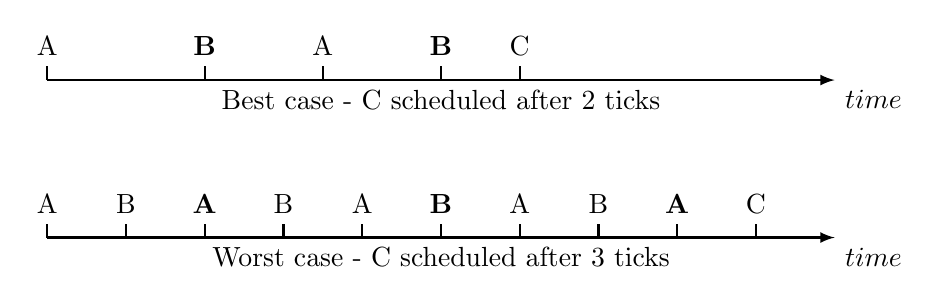
\begin{tikzpicture}[x=1cm]

          \draw[->,thick,>=latex] (0,0) -- (10,0) node[below right] {$time$};
          \draw[thick] (0,0) -- ++(0,5pt) node[above] {A};
          \draw[thick] (1,0) -- ++(0,5pt) node[above] {B};
          \draw[thick] (2,0) -- ++(0,5pt) node[above] {\textbf{A}};
          \draw[thick] (3,0) -- ++(0,5pt) node[above] {B};
          \draw[thick] (4,0) -- ++(0,5pt) node[above] {A};
          \draw[thick] (5,0) -- ++(0,5pt) node[above] {\textbf{B}};
          \draw[thick] (6,0) -- ++(0,5pt) node[above] {A};
          \draw[thick] (7,0) -- ++(0,5pt) node[above] {B};
          \draw[thick] (8,0) -- ++(0,5pt) node[above] {\textbf{A}};
          \draw[thick] (9,0) -- ++(0,5pt) node[above] {C};

          \node[below,align=left,anchor=north,inner xsep=0pt] at (5,0)
              {Worst case - C scheduled after 3 ticks};

          \draw[->,thick,>=latex] (0,2) -- (10,2) node[below right] {$time$};
          \draw[thick] (0,2) -- ++(0,5pt) node[above] {A};
          \draw[thick] (2,2) -- ++(0,5pt) node[above] {\textbf{B}};
          \draw[thick] (3.5,2) -- ++(0,5pt) node[above] {A};
          \draw[thick] (5,2) -- ++(0,5pt) node[above] {\textbf{B}};
          \draw[thick] (6,2) -- ++(0,5pt) node[above] {C};

          \node[below,align=left,anchor=north,inner xsep=0pt] at (5,2)
              {Best case - C scheduled after 2 ticks};
      \end{tikzpicture}
      \caption{Scheduling in the case of IPC and variable execution times. A
and B are IPC partners, C is a third thread. A, B and C run at the same
priority. All threads have a timeslice of 5. Bold indicates the thread that is
preempted by the timer tick. In the best case, B takes both timer ticks and C
is scheduled after 5 ticks. In the worst case, A takes 4 ticks and B takes 5,
such that C is scheduled after 9 ticks.} \label{fig:non-determinism}
  \end{figure}

\subsection{Capabilities to time}
\label{s:capabilities}

Capabilities~\citep{Dennis_VanHorn_66} are an established mechanism for
fine-grained access control to spatial resources. The  \selfour
microkernel uses capabilities to provide a memory-management model
that delegates all management decisions to user level,
including allocation of kernel memory, resulting in a largely
policy-free
kernel~\citep{Elkaduwe_DE_08,Heiser_Elphinstone_16}.
However, the capability system in \selfour does not presently apply to time.

Many existing and research \glspl{OS} use capabilities for a variety of things. \composite, NOVA,
KeyKOS, EROS, Fiasco O.C and Barrelfish all provide capability systems. 

Prior uses of capabilities for controlling time include
KeyKOS~\citep{Bomberger_FFHLS_92}, which had capabilities to \emph{meters}, which granted the holder
the right to execute for the unit of time held by the meter.
However, the KeyKOS model treats time as fungible, with no guarantee
of \emph{when} the time will be provided, which makes this approach
unsuitable for real-time use.

EROS~\citep{Shapiro_SF_99} combined processor capacity reserves with capabilities rather than the
meters of KeyKOS. However these reserves were optional: a two level scheduler first
scheduled the reserves with available capacity, then threads with no
or exhausted reserves were scheduled.
Like any hierarchical scheduling model, this enforces a policy that
reduces flexibility.

Furthermore, hierarchical delegation has the significant disadvantage
of algorithmic utilisation loss~\citep{Lackorzynski_WVH_12}; this is a
direct result of the unfungible nature of time. Consider real
estate: like time, it is (arbitrarily) divisible but not fungible: If
a block is too small to build a house, then having a second,
disconnected block of the same size is of no help (unlike spatial resources in a kernel, which can
be mapped side-by-side). The implication is
that capabilities for time have a different flavour from those for
spatial resources -- they cannot support hierarchical delegation
without loss, and cannot be recursively virtualised. While delegation is an
attractive property of spatial capabilities,
this delegation is not their defining characteristic, which is actually
\emph{prima facie evidence of access}; in the case of time
capabilities, the access is to processor time.

\composite recently introduced temporal capabilities
(tCaps)~\citep{Gadepalli_GBKP_17} reminiscent of
the meters of KeyKOS in that they represent a scalar unit of time.
Unlike KeyKOS, tCaps integrate with user-level scheduling, decoupling access control
from scheduling. An initial capability \emph{chronos} provides authority to all of time, and this capability
can used to replenish tCaps by a top level scheduler. The kernel up calls user-level schedulers 
which must then provide a tCap and a thread to execute. A tCap is always active in the system with
any time billed to it. The top level scheduler delegates fixed amounts of time from the initial,
infinite tCap, which can then be further delegated and split according to the scheduling policy,
which could be simple fixed-priority or a more complex scheduling hierarchy, such as that presented
in \hires~\citep{Parmer_West_11}. If all time
in a tCap is depleted, other, non-depleted tCaps will be scheduled until eventually the top level
tCap is scheduled. For efficiency, tCap delegation is limited to a constant of 16. 

\section{Summary}

In this chapter we have reviewed existing real-time operating systems and techniques applicable to
treating time as a first class resource, as part of our goal to design microkernel mechanisms for 
the support of mixed-criticality workloads. 
As we have seen, many existing systems conflate criticality and time sensitivity 
in a single value: priority. A further assumption is that high criticality, time sensitive tasks are
always trusted, one the falls apart in the mixed criticality context.

The \emph{criticality} of a component reflects its importance to the
overall system mission.
Criticality may reflect the impact of failure~\citep{ARINC653} or the
utility of a function. An MCS should degrade gracefully, with
components of lower criticality (which we will for simplicity refer to
as \crit{low} components) suffering degradation before higher
criticality (\crit{high}) components.

\emph{Time sensitivity} refers to how important it is to a thread to
get access to the processor at a particular time. For best-effort activities, time is
fungible, in that only the amount of time allocated is of
relevance. In contrast, for a hard real-time component, time is
largely unfungible, in that the allocation has no value if it occurs after
the deadline; soft real-time components are in between.

Finally, \emph{trust} refers to the degree of reliance in the correct
behaviour of a component. Untrusted components may fail completely
without affecting the core system mission, while a component which
must be assumed to operate correctly for achieving the overall mission
is trusted. A component is \emph{trustworthy} if it has undergone a process
that establishes that it can be trusted, the degree of trustworthiness
being a reflection of the rigour of this process (testing,
certification, formal verification)~\citep{Verissimo_NC_03}.
\Cref{plot:ternary} illustrates these axis.

\begin{figure}
    \centering
    \begin{tikzpicture}
        \begin{ternaryaxis}[
            xlabel=Criticality,
            ylabel=Trustworthiness,
            zlabel=Real-time sensitivity,
            label style=sloped,]
        \end{ternaryaxis}
    \end{tikzpicture}
    \caption{Commonly conflated attributes of systems software}
    \label{plot:ternary}
\end{figure}

In practice, criticality and trust are closely aligned, as the most
critical parts should be the most trustworthy.
However, criticality must be decoupled from time sensitivity in MCS.
Referring back to the
example in the introduction, interrupts from networks or buses have
high time sensitivity, but low criticality (i.e.\ deadline misses are
tolerable), while the opposite is true for the flight control component.
Similarly, threads (other than the most critical ones which should
have undergone extensive assurance) cannot be
trusted to honour their declared WCET.

Our claim is that how these attributes are conflated is
policy that is specific to a system.
We need a mechanism that allows  enforcing time limits, and thus
isolate the timeliness of critical threads from those of untrusted,
less critical ones.
Reservation-based kernels often allow for a form of over-committing where
best-effort threads are run in the slack-time left by unused reservations or unreserved CPU.
However this also aligns criticality and time-sensitivity, and
enforces a two-level scheduling model.

If trustworthiness and real-time sensitivity are not conflated, many assumptions about real-time
scheduling fail.
Much real-time analysis rely on threads having a known \gls{WCET}, which implies that those threads
are predictable, which implies trust.
If a real-time thread is not expected to behave correctly, one cannot
assume it will surrender access to the processor voluntarily.
Consequently, the \gls{PIP}/\gls{BWI} based scheduling-context donation mechanisms seen in this chapter are
insufficient, forcing not only a protocol which causes extensive preemption overhead, but 
requiring shared servers to have known, bounded execution time on all requests.

In the next chapter we present a model for mixed-criticality scheduling that is suitable for high
assurance systems such as \selfour. 
